\documentclass[conference]{IEEEtran}
% Required Packages
\IEEEoverridecommandlockouts
\usepackage{graphicx}
\usepackage{amsmath}
\usepackage{cite}
\usepackage{url}
\usepackage{booktabs}
\usepackage{float}
\usepackage{amsmath}
\usepackage{hyperref}
\usepackage{amssymb}
\usepackage[skip=5pt]{caption}
\usepackage{subfigure}
\usepackage{hyperref}
\usepackage{cleveref}  % smart referencing


  \makeatletter
\newcommand{\linebreakand}{%
  \end{@IEEEauthorhalign}
  \hfill\mbox{}\par
  \mbox{}\hfill\begin{@IEEEauthorhalign}
}
\makeatother
\IEEEpubid{\begin{minipage}[t]{\textwidth}\ \\[10pt]
      \normalsize{  979-8-3315-1504-1/25/\$31.00 ©2025 IEEE} 
\end{minipage}}



\begin{document}

\title{Uncertainty-Aware Multimodal Deep Learning Framework for Stress Detection Using Audio-Visual Signals}

% Author Information
\author{
 \IEEEauthorblockN{Meruva Kodanda Suraj}
     \IEEEauthorblockA{
 Department of DSAI\\
   IIIT Naya Raipur, Chhattisgarh, India\\
        Email: meruva24102@iiitnr.edu.in \\
    }

     \and
    \IEEEauthorblockN{Mamta Nag}
    \IEEEauthorblockA{
        Department of CSE\\
        IIIT Naya Raipur, Chhattisgarh, India\\
        Email: mamta@iiitnr.edu.in\\
    }

 
    \and
    \IEEEauthorblockN{ Mallikharjuna Rao K}
     \IEEEauthorblockA{
 Department of DSAI\\
   IIIT Naya Raipur, Chhattisgarh, India\\
        Email: mallikharjuna@iiitnr.edu.in\\
    }
     
}


% Create the title
\maketitle

% Abstract
\begin{abstract}
Multimodal stress detection systems have demonstrated strong classification performance using deep learning architectures. However, existing models provide deterministic predictions without quantifying predictive uncertainty or evaluating calibration quality, limiting their reliability in clinical and occupational deployment. This paper proposes an uncertainty-aware, confidence-calibrated multimodal stress detection framework built upon a hybrid 3D-CNN + EfficientNet-B0 + Action Unit (AU) gating architecture. Using the RAVDESS dataset, the proposed extension integrates Monte Carlo Dropout, temperature scaling, test-time augmentation, and selective prediction. The framework produces calibrated probabilities, quantifies predictive uncertainty, and enables abstention on ambiguous samples. Experimental results demonstrate improved reliability, reduced overconfidence, and enhanced selective risk control while maintaining strong recall for stress detection.  
\end{abstract}
\begin{IEEEkeywords}
Stress Detection, Multimodal Learning, Uncertainty Estimation, Monte Carlo Dropout, Temperature Scaling
\end{IEEEkeywords}
% Introduction Section
\section{Introduction}

Stress is an increasingly critical concern in modern society, particularly in high-demand occupational and clinical environments where prolonged psychological pressure can lead to anxiety disorders, depression, cardiovascular complications, and reduced cognitive performance. Persistent stress not only affects individual well-being but also impacts professional productivity and decision-making quality. Early detection and accurate categorization of stress states are therefore essential for preventive healthcare, workplace safety, and mental health intervention strategies \cite{ref1,ref2,ref3}.
Traditional stress assessment methods, such as self-reported questionnaires, interviews, and psychological scoring systems, often suffer from subjectivity, delayed reporting, and limited real-time applicability \cite{ref4,ref5}. These approaches rely heavily on personal perception and may fail to capture subtle physiological and behavioral variations associated with stress responses. Consequently, there is a growing demand for automated, objective, and real-time stress detection systems capable of continuous monitoring.
Recent advancements in deep learning and affective computing have enabled the development of intelligent stress recognition systems that analyze multimodal signals, including facial expressions and speech patterns. Audio-visual datasets such as RAVDESS facilitate structured modeling of emotion-related stress states through synchronized speech and facial recordings \cite{ref5}. Deep neural networks, particularly convolutional and spatio-temporal architectures, have demonstrated strong capability in extracting discriminative representations from facial dynamics and acoustic features \cite{ref6,ref7,ref8}. These data-driven approaches enhance stress detection accuracy while reducing biases inherent in subjective evaluations.
To improve multimodal prediction performance, this study employs a hybrid deep learning framework combining 3D convolutional neural networks for spatio-temporal facial modeling and EfficientNet-B0 for high-level spatial feature extraction, integrated with an Action Unit (AU) gating mechanism and an audio convolutional branch. Unlike traditional deterministic classifiers, the proposed system further incorporates uncertainty-aware mechanisms to improve reliability and deployment safety.

The proposed framework extends conventional multimodal stress classification by integrating Monte Carlo Dropout for predictive uncertainty estimation, temperature scaling for confidence calibration, test-time augmentation for robustness enhancement, and selective prediction for abstention on ambiguous samples. Monte Carlo Dropout approximates Bayesian inference through stochastic forward passes, enabling computation of predictive mean and variance. Temperature scaling corrects overconfident probability estimates without affecting classification accuracy. Selective prediction mechanisms allow the system to reject high-uncertainty predictions, thereby improving reliability in safety-critical environments.
Experimental evaluation compares baseline CNN-LSTM, transformer-based cross-attention, and the proposed hybrid architecture. Results demonstrate that while stress detection recall remains high, the integration of uncertainty estimation and calibration significantly improves model trustworthiness, reduces overconfidence, and enhances selective performance under uncertainty constraints.
This study contributes to the development of reliable AI-driven stress monitoring systems capable of producing calibrated probabilistic outputs and uncertainty-aware decisions. Such systems are particularly relevant for workplace stress monitoring, telehealth platforms, and preventive mental health screening. Future research may explore conformal prediction frameworks, out-of-distribution detection, and real-time deployment using edge-based multimodal sensing systems.

\section{Related Works}
Stress detection using artificial intelligence techniques has gained significant attention in recent years, particularly in healthcare and occupational environments. Iqbal et al.~\cite{ref1} demonstrated the effectiveness of wearable sensors for stress monitoring and emphasized the importance of physiological signals for real-time stress prediction. Their study employed advanced sensor-based systems to collect multimodal physiological data, enabling early stress identification. However, substantial inter-individual variability in physiological responses limited the generalizability of their findings, highlighting the need for adaptive and personalized stress detection models.
Awada et al.~\cite{ref2} introduced an automated framework to distinguish between eustress and distress, providing deeper insight into the psychological dimensions of stress analysis. Their approach emphasized differentiating beneficial stress from harmful stress for targeted interventions. Nevertheless, the study faced challenges related to limited labeled data availability and relied on semi-supervised learning strategies to mitigate data scarcity issues.
Hosseini et al.~\cite{ref3} proposed a multimodal dataset for continuous stress detection in nurses, integrating various physiological signals to improve classification performance. Their findings indicated that combining multiple physiological markers enhances predictive accuracy. However, class imbalance, where stress samples were underrepresented, negatively affected model training and introduced potential bias in classification outcomes.

Gedam and Paul~\cite{ref4} conducted a comprehensive review of wearable sensor-based stress detection systems, comparing various machine learning algorithms. Their analysis showed that ensemble-based methods such as Random Forest and gradient boosting models generally achieved superior performance. Despite promising results, they identified computational complexity and limited real-time adaptability as major constraints, particularly in resource-constrained environments.
Beyond physiological sensing, Nijhawan et al.~\cite{ref5} explored stress detection using textual features derived from social media interactions. Their findings demonstrated that linguistic patterns and emotional fluctuations in text could serve as stress indicators. However, contextual ambiguity and the complexity of stress-related expressions often led to misinterpretations, underscoring the need for more advanced natural language processing techniques.
Similarly, Rastogi et al.~\cite{ref6} introduced a benchmark dataset for social media-based stress detection and highlighted the complementary role of textual features alongside physiological signals. Although their approach improved stress recognition capability, inconsistencies and variability in social media content limited model robustness and real-world generalizability.

Bobade et al.~\cite{ref7} investigated multimodal stress detection using both machine learning and deep learning architectures, including CNNs and LSTMs. Their study demonstrated that deep learning models effectively extract discriminative features from physiological signals. However, high computational costs and limited interpretability of deep models posed challenges for real-world deployment, particularly in healthcare applications requiring transparency and reliability.
Zhu et al.~\cite{ref8} reinforced the importance of multimodal fusion strategies by integrating multiple biometric inputs to enhance stress detection accuracy. While fusion improved classification performance, heavy reliance on sensor precision made the system vulnerable to noise and signal degradation. Additionally, wearable-based approaches may face compliance issues due to user discomfort.
Moosavi et al.~\cite{ref9} proposed a deep learning framework incorporating Q-learning optimization for early stress detection. Although the approach achieved improved predictive accuracy, the model complexity and computational requirements limited its practicality for real-time implementation.
Saylam et al.~\cite{ref10} examined digital biomarkers for stress and anxiety prediction using wearable devices. Their results showed promising time-dependent prediction capability; however, differentiating between physiologically similar states, such as anxiety and physical exertion, remained a significant challenge.
Sharma et al.~\cite{ref11} conducted a comparative evaluation of conventional machine learning algorithms for stress level detection. While their study provided valuable insights into classification performance, they emphasized the need for explainable AI techniques to enhance transparency and trust in medical and clinical decision-making systems.

\subsection{Research Gap}

Despite extensive research in physiological, textual, and multimodal stress detection, several limitations persist. Existing approaches primarily rely on wearable sensors or textual analysis, which may suffer from noise, compliance issues, contextual ambiguity, and data imbalance. Furthermore, many deep learning models provide deterministic predictions without quantifying predictive uncertainty or ensuring probability calibration. The absence of uncertainty estimation and confidence-aware decision mechanisms limits their reliability for safety-critical and healthcare-related deployments.

To address these limitations, the present study focuses on multimodal audio-visual stress detection with uncertainty quantification and confidence calibration, aiming to enhance reliability, robustness, and real-world applicability.

\section{Stress Prediction Model Overview}

\subsection{Purpose}

The purpose of the proposed model is to develop a robust multimodal framework for automatic stress detection using facial expressions and speech signals. Traditional unimodal stress detection systems rely on either visual or acoustic information, which often results in limited performance due to missing contextual cues. To address this limitation, the proposed framework integrates facial video features and speech-based acoustic representations using a hybrid deep learning architecture.

The system combines a 3D Convolutional Neural Network (3D-CNN) for capturing spatial–temporal facial dynamics and EfficientNet-B0 for extracting high-level spatial representations from facial frames. By integrating visual and acoustic modalities, the framework aims to improve stress recognition performance and provide a more reliable classification of stress states.

\subsection{System Workflow}

The proposed multimodal stress detection framework is illustrated in Figure~\ref{fig:sample}. The system follows a structured pipeline consisting of data acquisition, preprocessing, feature extraction, multimodal fusion, and classification.

Initially, the RAVDESS dataset containing audio–visual recordings of emotional speech expressions is used as the primary data source. The dataset includes synchronized facial video frames and corresponding speech signals. Preprocessing steps such as frame extraction, face detection, audio normalization, and temporal segmentation are applied to ensure high-quality input data.

For visual analysis, facial frames are processed using a hybrid deep learning architecture that combines 3D-CNN and EfficientNet-B0 to capture both temporal motion dynamics and spatial facial representations. In parallel, acoustic features are extracted from speech signals to capture vocal characteristics associated with stress.

The extracted visual and acoustic features are fused using a multimodal feature fusion strategy. The fused representation is then passed through fully connected layers for final classification. The output layer predicts two categories: \textit{Stress} and \textit{Non-Stress}.

\begin{figure*}[t]
    \centering
    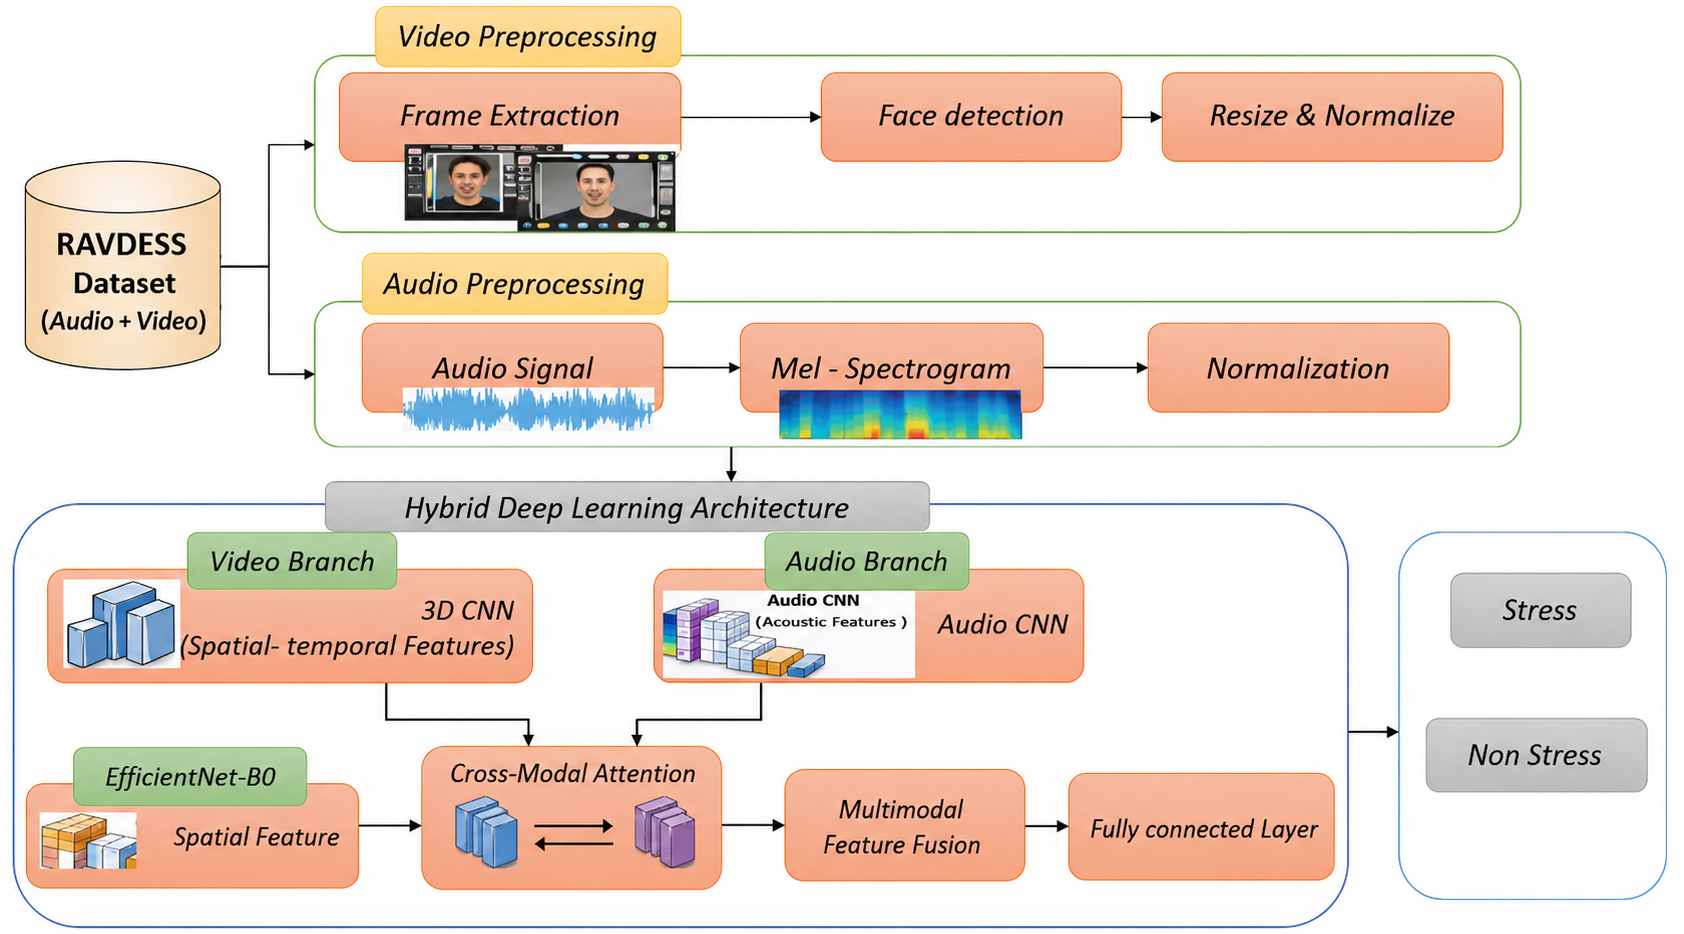
\includegraphics[width=0.75\textwidth]{pro.png}
    \caption{Proposed Multimodal Stress Detection Framework}
    \label{fig:sample}
\end{figure*}

\subsection{Dataset}

This study utilizes the publicly available RAVDESS (Ryerson Audio-Visual Database of Emotional Speech and Song) dataset, which is widely used in emotion recognition research. The dataset contains audio–visual recordings of emotional speech performed by 24 professional actors (12 male and 12 female).

Each actor expresses eight emotional states including neutral, calm, happy, sad, angry, fearful, disgust, and surprise. The recordings consist of high-quality video clips with synchronized speech signals.

For stress detection, emotions such as anger, fear, and sadness are considered stress-related categories, while neutral and calm expressions are treated as non-stress states.

\subsection{Data Preprocessing}

Effective preprocessing is essential for improving model performance and ensuring reliable stress detection. The preprocessing pipeline includes facial frame extraction, face detection, image resizing, and normalization.

Video clips are decomposed into frame sequences, and facial regions are detected and extracted. All images are resized to a consistent resolution to ensure compatibility with deep learning models.

For the audio modality, speech signals are normalized and converted into Mel-spectrogram representations. These time–frequency representations capture important acoustic characteristics related to emotional stress.

\subsection{Data Segmentation}

Temporal segmentation is applied to divide video sequences into smaller clips while preserving motion information. Each video sample is segmented into fixed-length frame sequences that allow the 3D-CNN model to capture temporal variations in facial expressions.

Similarly, audio signals are segmented into short time windows to generate spectrogram representations that capture speech dynamics associated with stress.

\subsection{Feature Extraction Using Deep Learning}

Deep learning architectures are employed to automatically extract discriminative features from visual and acoustic modalities.

\begin{itemize}

\item \textbf{3D Convolutional Neural Network (3D-CNN)}

The 3D-CNN model extracts spatio-temporal features from facial video sequences. Unlike conventional 2D CNNs, 3D-CNNs perform convolution across spatial and temporal dimensions simultaneously.

\begin{equation}
F_{out}(x,y,t) = \sum_{i}\sum_{j}\sum_{k} W(i,j,k) \cdot X(x+i,y+j,t+k)
\end{equation}

where $X$ represents the input feature volume and $W$ denotes the learnable 3D convolution kernel.

\item \textbf{EfficientNet-B0}

EfficientNet-B0 is utilized to extract high-level spatial features from facial frames. EfficientNet employs compound scaling to balance network depth, width, and input resolution.

\begin{equation}
Depth = \alpha^{\phi}, \quad Width = \beta^{\phi}, \quad Resolution = \gamma^{\phi}
\end{equation}

subject to

\begin{equation}
\alpha \cdot \beta^2 \cdot \gamma^2 \approx 2
\end{equation}

where $\phi$ controls the scaling coefficient of the network.

\end{itemize}

\subsection{Multimodal Feature Fusion}

To utilize complementary information from facial and speech modalities, feature-level fusion is applied. The extracted visual and audio feature vectors are concatenated to form a unified representation.

\begin{equation}
F_{fusion} = [F_{visual} \oplus F_{audio}]
\end{equation}

where $\oplus$ represents feature concatenation.

This multimodal representation enables the model to capture both facial expression dynamics and speech characteristics associated with stress.

\subsection{Model Training and Stress Classification}

The fused feature vector is passed through fully connected layers for classification. The final prediction layer uses the Softmax activation function to compute the probability distribution over stress classes.

\begin{equation}
P(y=k|x) = \frac{e^{z_k}}{\sum_{j=1}^{K} e^{z_j}}
\end{equation}

Since the task is binary classification, the final output corresponds to two classes: \textit{Stress} and \textit{Non-Stress}.
The model parameters are optimized using backpropagation during training. Performance evaluation is conducted using standard metrics including accuracy, precision, recall, F1-score, and Area Under the Curve (AUC).

\section{Results and Discussion}
This section presents a comprehensive evaluation of , which integrates the Hybrid (3D-CNN + EfficientNet-B0 + AU) architecture with uncertainty estimation and probability calibration. The evaluation focuses on three key aspects: classification performance, calibration quality, and uncertainty-aware prediction behavior.

\subsubsection{Overall Classification Performance}

Table~\ref{tab:all_arch_comparison} presents a comparative performance analysis across all evaluated architectures, including the baseline CNN–LSTM model, the cross-attention dual-stream model, the deterministic Hybrid architecture, and the proposed framework.
While the deterministic Hybrid model achieves slightly higher raw accuracy, This introduces probabilistic calibration and uncertainty estimation that significantly enhance the reliability and interpretability of predictions. The proposed framework therefore prioritizes trustworthy predictions rather than maximizing point-estimate accuracy alone.

\begin{table}[H]
\centering
\caption{Performance Comparison Across All Architectures}
\label{tab:all_arch_comparison}
\footnotesize
\setlength{\tabcolsep}{2pt}
\renewcommand{\arraystretch}{1.0}
\begin{tabular}{lccccc}
\hline
\textbf{Model} & \textbf{Acc.} & \textbf{Prec.} & \textbf{Recall} & \textbf{F1} & \textbf{AUC} \\
\hline
Baseline (CNN-2D + LSTM) & 0.885 & 0.860 & 0.920 & 0.889 & 0.971 \\
Cross-Attention (Dual-Stream) & 0.790 & 0.790 & 0.790 & 0.790 & 0.890 \\
Hybrid (3D-CNN + EffNet-B0 + AU) & 0.850 & 0.802 & 0.930 & 0.861 & 0.940 \\
\textbf{ (Hybrid + Uncertainty)} & \textbf{0.813} & \textbf{0.783} & \textbf{0.867} & \textbf{0.823} & \textbf{0.878} \\
\hline
\end{tabular}
\end{table}

To further illustrate this trade-off, Table~\ref{tab:hybrid_vs_pipelineD} provides a direct comparison between the deterministic Hybrid model and the uncertainty-aware . The results indicate that while the deterministic model achieves marginally higher accuracy,  enables calibrated confidence estimates that are crucial for reliable deployment in safety-critical applications.

\begin{table}[H]
\centering
\caption{Classification Performance: Hybrid vs }
\label{tab:hybrid_vs_pipelineD}
\footnotesize
\setlength{\tabcolsep}{4pt}
\renewcommand{\arraystretch}{1.0}
\begin{tabular}{lcc}
\hline
\textbf{Metric} & \textbf{Hybrid} & \textbf{} \\
\hline
Accuracy & 0.850 & 0.813 \\
Recall  & 0.930 & 0.867 \\
F1      & 0.861 & 0.823 \\
AUC     & 0.940 & 0.878 \\
\hline
\end{tabular}
\end{table}

\subsubsection{Per-Class Performance}

Table~\ref{tab:perclass_pipelineD} presents the per-class classification report for  on the balanced test set consisting of 150 samples (75 stress and 75 non-stress). The results indicate slightly stronger detection performance for the non-stress class, while maintaining balanced macro and weighted averages across precision, recall, and F1-score.

\begin{table}[H]
\centering
\caption{Per-Class Classification Report ()}
\label{tab:perclass_pipelineD}
\footnotesize
\setlength{\tabcolsep}{3pt}
\renewcommand{\arraystretch}{1.0}
\begin{tabular}{lcccc}
\hline
\textbf{Class} & \textbf{Precision} & \textbf{Recall} & \textbf{F1 Score} & \textbf{Support} \\
\hline
Stress     & 0.8500 & 0.7600 & 0.8000 & 75 \\
Non-Stress & 0.7800 & 0.8700 & 0.8200 & 75 \\
\textbf{Macro Avg}    & \textbf{0.8200} & \textbf{0.8100} & \textbf{0.8100} & \textbf{150} \\
\textbf{Weighted Avg} & \textbf{0.8200} & \textbf{0.8100} & \textbf{0.8100} & \textbf{150} \\
\hline
\end{tabular}
\end{table}

The confusion matrix shown in Fig.~\ref{fig:pipd_confmat} provides a detailed view of classification outcomes. Out of 150 test samples, 122 samples are correctly classified, while 28 samples are misclassified.

\begin{figure}[H]
\centering
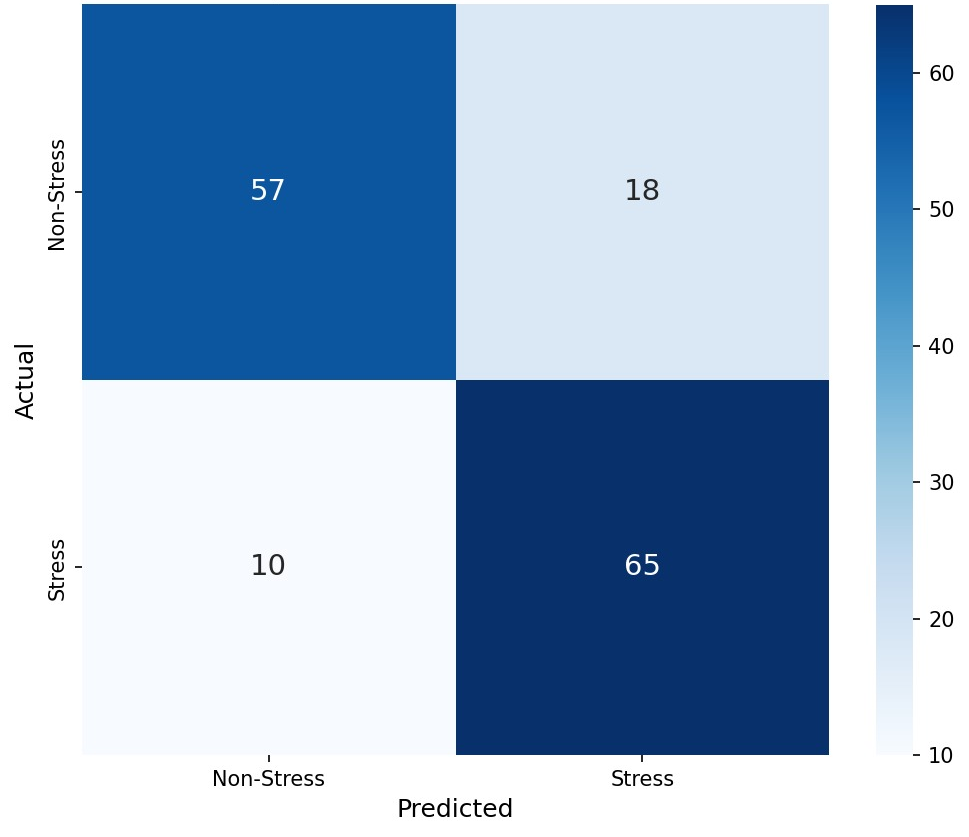
\includegraphics[width=0.9\linewidth]{confusion_matrix.png}
\caption{Confusion Matrix for .}
\label{fig:pipd_confmat}
\end{figure}

\subsubsection{Calibration Performance}

A key component of  is probability calibration through temperature scaling. Table~\ref{tab:calibration_metrics} presents calibration metrics before and after scaling with a learned temperature parameter of $T = 3.0855$.

Temperature scaling significantly improves calibration quality, reducing Expected Calibration Error (ECE) by nearly 60\% and Maximum Calibration Error (MCE) by approximately 67\%.

\begin{table}[H]
\centering
\caption{Calibration Metrics Before and After Temperature Scaling}
\label{tab:calibration_metrics}
\footnotesize
\setlength{\tabcolsep}{2.5pt}
\renewcommand{\arraystretch}{1.0}
\begin{tabular}{lccc}
\hline
Metric & Before & After & Improvement \\
\hline
ECE & 0.1768 & \textbf{0.0710} & $\downarrow$ 59.8\% \\
MCE & 0.7651 & \textbf{0.2531} & $\downarrow$ 66.9\% \\
Brier Score & 0.1734 & \textbf{0.1450} & $\downarrow$ 16.4\% \\
NLL & 0.7172 & \textbf{0.3940} & $\downarrow$ 45.1\% \\
\hline
\end{tabular}
\end{table}

Figure~\ref{fig:tempscale} further illustrates this improvement using reliability diagrams before and after calibration.

\begin{figure}[H]
\centering
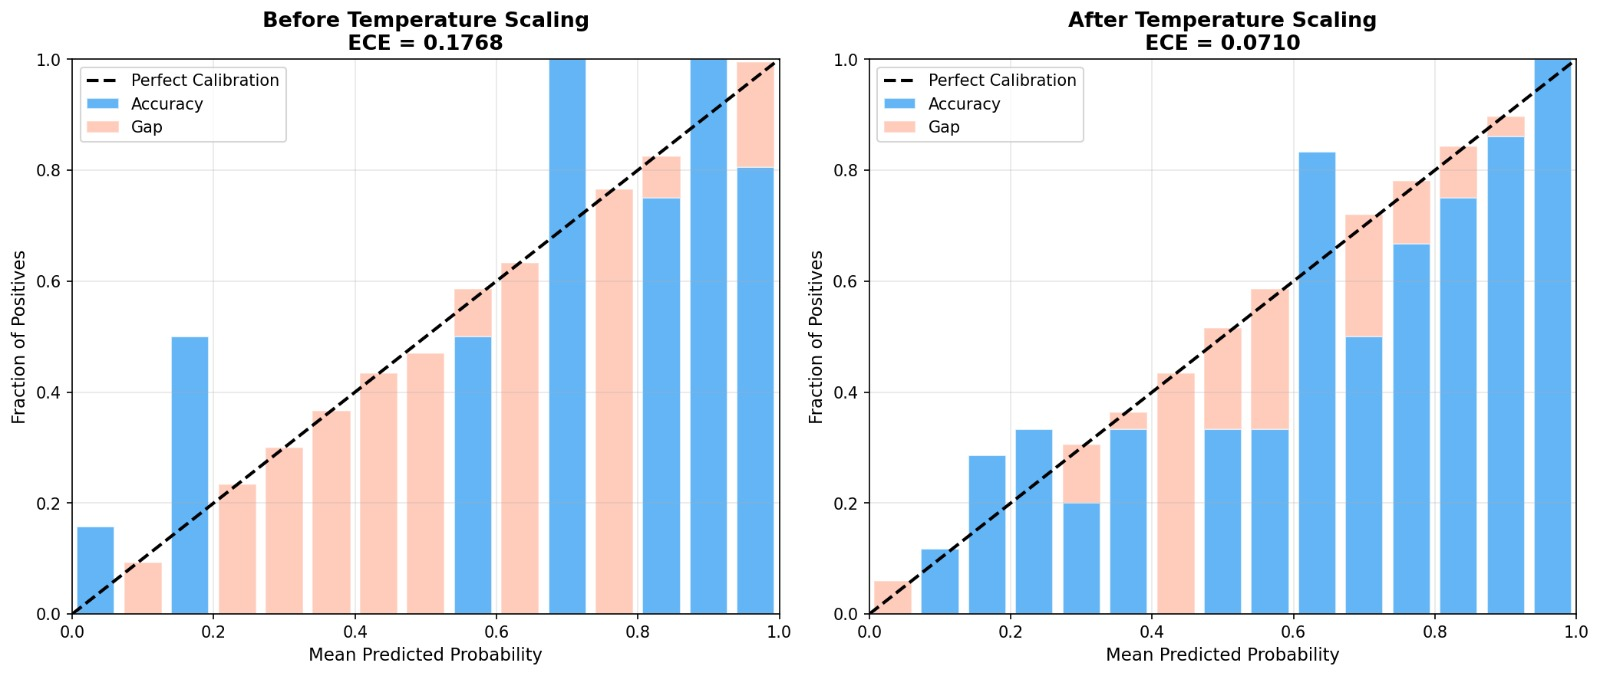
\includegraphics[width=\linewidth]{reliability_diagram.png}
\caption{Reliability diagrams before and after temperature scaling.}
\label{fig:tempscale}
\end{figure}

\subsubsection{Uncertainty Estimation Analysis}

Uncertainty estimation is performed using Monte Carlo Dropout with $T = 20$ stochastic forward passes. Table~\ref{tab:uncertainty_stats} summarizes key uncertainty metrics, including predictive variance, entropy, and the Uncertainty AUROC.

\begin{table}[H]
\centering
\caption{Uncertainty Estimation Statistics}
\label{tab:uncertainty_stats}
\footnotesize
\setlength{\tabcolsep}{3pt}
\renewcommand{\arraystretch}{1.0}
\begin{tabular}{lc}
\hline
Metric & Value \\
\hline
Mean Predictive Variance & 0.001564 \\
Mean Predictive Entropy & 0.1092 \\
Uncertainty AUROC & 0.6906 \\
Risk-Coverage AURC & 0.1015 \\
\hline
\end{tabular}
\end{table}

The uncertainty distribution shown in Fig.~\ref{fig:uncert} confirms that misclassified samples tend to exhibit higher predictive variance than correctly classified samples.

\begin{figure}[H]
\centering
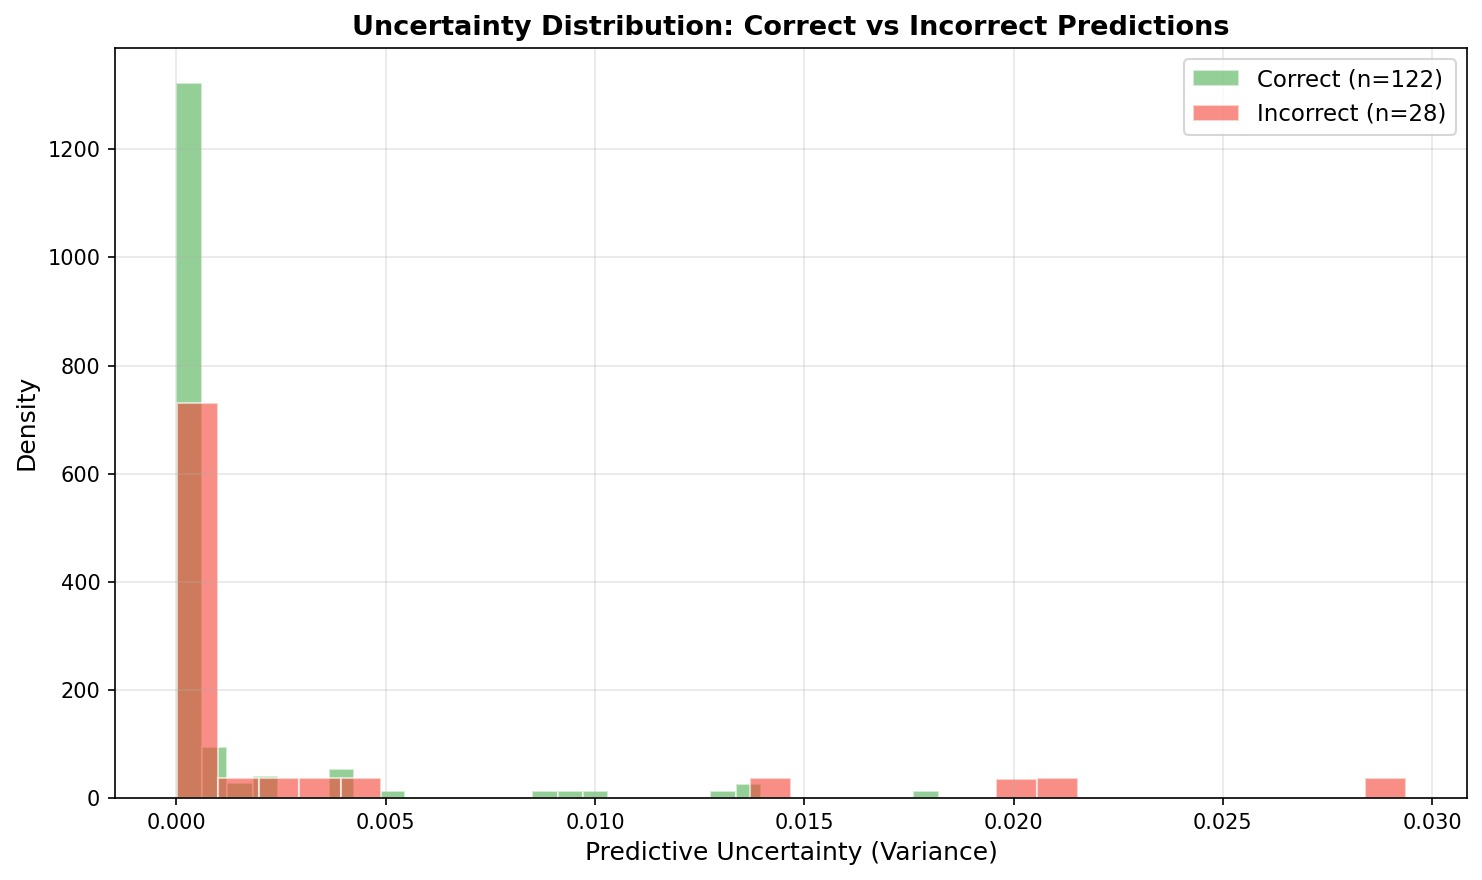
\includegraphics[width=0.9\linewidth]{uncertainty_distribution.png}
\caption{Predictive uncertainty distribution for correct and incorrect predictions.}
\label{fig:uncert}
\end{figure}

\subsubsection{Selective Prediction Performance}

Selective prediction experiments evaluate the impact of rejecting uncertain samples. Table~\ref{tab:selective_pred_full} shows that increasing the rejection rate gradually improves classification performance.

\begin{table*}[htbp]
\centering
\caption{Selective Prediction Performance at Different Rejection Levels}
\label{tab:selective_pred_full}
\footnotesize
\setlength{\tabcolsep}{4pt}
\renewcommand{\arraystretch}{1.0}
\begin{tabular}{lccccccc}
\hline
Rejection Rate & Kept & Rejected & Accuracy & Precision & Recall & F1 Score & AUC \\
\hline
0\% & 150 & 0  & 0.8133 & 0.7831 & 0.8667 & 0.8228 & 0.8782 \\
5\% & 143 & 7  & 0.8322 & 0.8077 & 0.8750 & 0.8400 & 0.8834 \\
10\% & 135 & 15 & 0.8296 & 0.8108 & 0.8696 & 0.8392 & 0.8887 \\
\textbf{20\%} & \textbf{120} & \textbf{30} & \textbf{0.8333} & \textbf{0.8088} & \textbf{0.8871} & \textbf{0.8462} & \textbf{0.8999} \\
\hline
\end{tabular}
\end{table*}

The risk-coverage curve shown in Fig.~\ref{fig:risk_curve} confirms that rejecting high-uncertainty samples significantly reduces prediction error.

\begin{figure}[H]
\centering
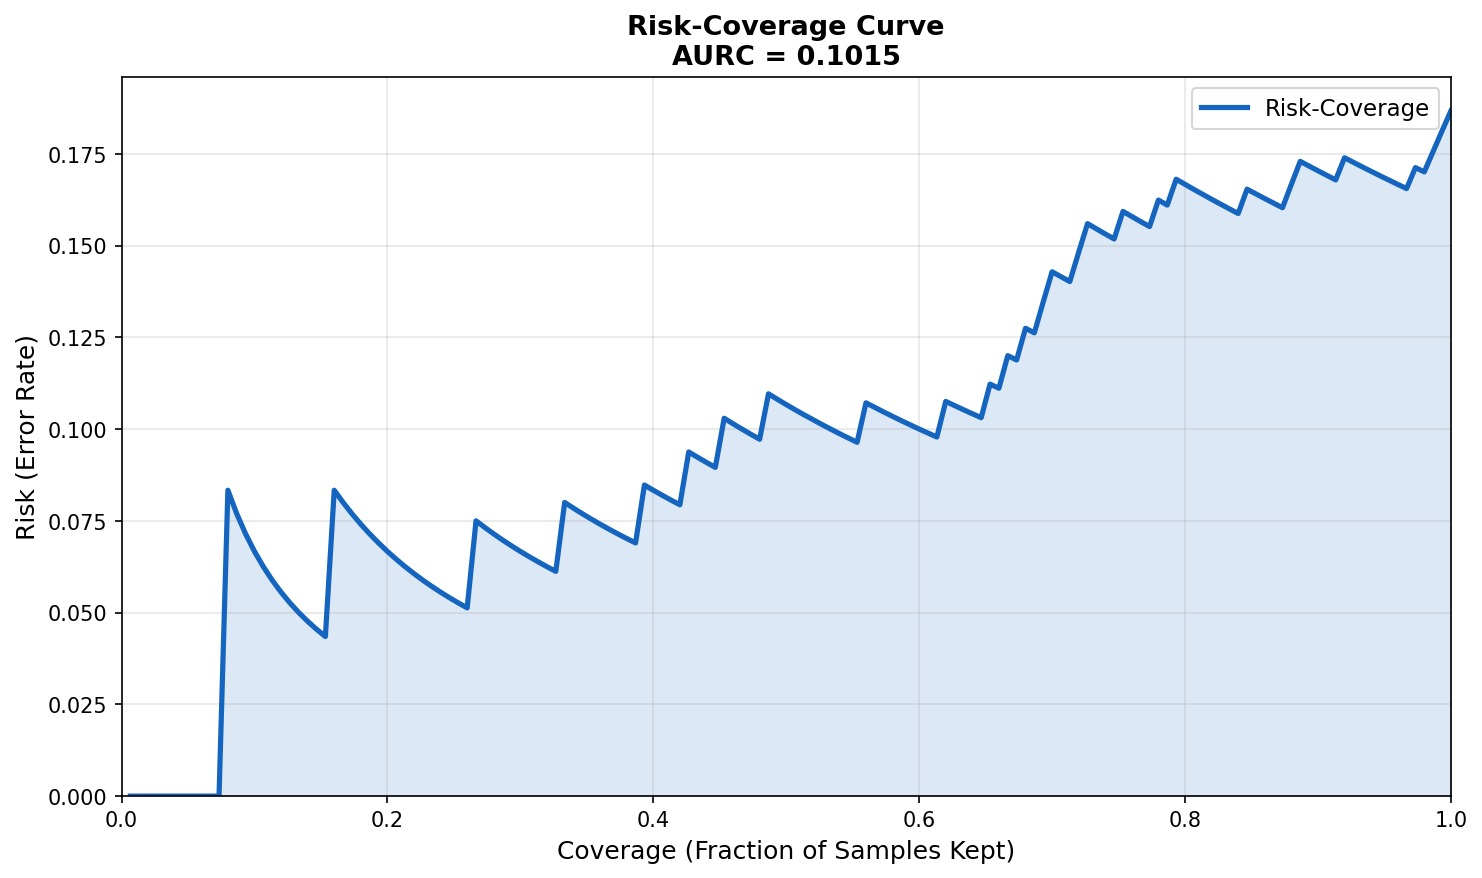
\includegraphics[width=0.9\linewidth]{risk_coverage.png}
\caption{Risk-Coverage Curve demonstrating uncertainty-aware error reduction.}
\label{fig:risk_curve}
\end{figure}

\subsubsection{Clinical Safety Analysis}

Table~\ref{tab:clinical_safety} evaluates stress recall under uncertainty constraints. As uncertain samples are excluded, recall for stress detection improves, which is critical in safety-sensitive monitoring applications.

\begin{table}[H]
\centering
\caption{Clinical Safety: Stress Recall under Uncertainty Constraints}
\label{tab:clinical_safety}
\footnotesize
\setlength{\tabcolsep}{3pt}
\renewcommand{\arraystretch}{1.0}
\begin{tabular}{lcc}
\hline
Condition & Recall (Stress) & Samples Evaluated \\
\hline
All samples & 0.8667 & 150 \\
Uncertainty $<$ median & 0.8750 & 143 \\
Uncertainty $<$ 75th percentile & 0.8696 & 135 \\
Uncertainty $<$ 80th percentile & \textbf{0.8871} & \textbf{120} \\
\hline
\end{tabular}
\end{table}

Overall, the results demonstrate that  successfully combines deep multimodal feature learning with uncertainty estimation and calibration, enabling reliable stress detection with improved prediction confidence and robustness.


\section{Limitations}

Although the proposed framework demonstrates promising performance, several limitations remain. 
First, the RAVDESS dataset contains acted emotional expressions rather than spontaneous real-world stress signals, which may affect generalization to real-world environments. 
Second, the dataset size is relatively small compared to large-scale deep learning datasets. 
Future work will investigate larger multimodal datasets and real-time deployment scenarios.
\section{Conclusion}

This paper presented an uncertainty-aware deep learning framework for facial stress detection that integrates hybrid feature learning, probabilistic calibration, and uncertainty estimation. The proposed  combines a Hybrid architecture consisting of 3D-CNN spatiotemporal encoding, EfficientNet-B0 spatial feature extraction, and Action Unit (AU) gating with Monte Carlo Dropout–based uncertainty estimation and temperature scaling for probability calibration.
Experimental evaluation on the RAVDESS dataset demonstrates that the proposed framework achieves strong classification performance while significantly improving prediction reliability.  achieved an accuracy of 0.8133 and an AUC of 0.8782 while providing calibrated probability estimates and interpretable uncertainty measures. Temperature scaling substantially improved calibration quality, reducing Expected Calibration Error (ECE) from 0.1768 to 0.0710 and decreasing negative log-likelihood by 45.1\%. These results indicate that the model’s predicted confidence better aligns with empirical accuracy after calibration.
Furthermore, uncertainty-aware selective prediction experiments show that rejecting uncertain samples improves overall system reliability. At a 20\% rejection rate, accuracy increased to 0.8333, recall improved to 0.8871, and AUC reached 0.8999. Risk–coverage analysis confirmed that Monte Carlo Dropout uncertainty effectively correlates with prediction errors, enabling the model to identify ambiguous or unreliable predictions. This behavior is particularly important for safety-critical applications where incorrect predictions may have serious consequences.
Overall, the proposed framework demonstrates that incorporating uncertainty estimation and probability calibration into deep stress detection models significantly improves their trustworthiness and deployment readiness. By enabling the system to quantify prediction confidence and abstain from uncertain decisions,  provides a practical foundation for reliable stress monitoring in healthcare, workplace well-being assessment, and human–computer interaction systems.

\begin{thebibliography}{99}
\bibitem{ref1}
Iqbal, Talha, et al. "Stress monitoring using wearable sensors: A pilot study and stress-predict dataset." Sensors 22.21 (2022): 8135.

\bibitem{ref2}
Awada, Mohamad, et al. "A new perspective on stress detection: An automated approach for detecting eustress and distress." IEEE Transactions on Affective Computing 15.3 (2023): 1153-1165.

\bibitem{ref3}
Hosseini, Seyedmajid, et al. "A multimodal sensor dataset for continuous stress detection of nurses in a hospital." Scientific Data 9.1 (2022): 255.

\bibitem{ref4}
Gedam, Shruti, and Sanchita Paul. "A review on mental stress detection using wearable sensors and machine learning techniques." IEEE Access 9 (2021): 84045-84066.

\bibitem{ref5}
Livingstone, Steven R., and Frank A. Russo. "The Ryerson Audio-Visual Database of Emotional Speech and Song (RAVDESS): A dynamic, multimodal set of facial and vocal expressions in North American English." PLoS ONE 13.5 (2018): e0196391.

\bibitem{ref6}
Tan, Mingxing, and Quoc V. Le. "EfficientNet: Rethinking model scaling for convolutional neural networks." Proceedings of the International Conference on Machine Learning (ICML). 2019.

\bibitem{ref7}
Gal, Yarin, and Zoubin Ghahramani. "Dropout as a Bayesian approximation: Representing model uncertainty in deep learning." Proceedings of the International Conference on Machine Learning (ICML). 2016.

\bibitem{ref8}
Guo, Chuan, et al. "On calibration of modern neural networks." Proceedings of the International Conference on Machine Learning (ICML). 2017.

\bibitem{ref9}
Lakshminarayanan, Balaji, Alexander Pritzel, and Charles Blundell. "Simple and scalable predictive uncertainty estimation using deep ensembles." Advances in Neural Information Processing Systems (NeurIPS). 2017.

\bibitem{ref10}
Geifman, Yonatan, and Ran El-Yaniv. "Selective classification for deep neural networks." Advances in Neural Information Processing Systems (NeurIPS). 2017.

\bibitem{ref11}
Kendall, Alex, and Yarin Gal. "What uncertainties do we need in Bayesian deep learning for computer vision?" Advances in Neural Information Processing Systems (NeurIPS). 2017.

\bibitem{ref12}
Carreira, Joao, and Andrew Zisserman. "Quo vadis, action recognition? A new model and the Kinetics dataset." Proceedings of the IEEE Conference on Computer Vision and Pattern Recognition (CVPR). 2017.

\bibitem{ref13}
Vaswani, Ashish, et al. "Attention is all you need." Advances in Neural Information Processing Systems (NeurIPS). 2017.

\bibitem{ref14}
Hochreiter, Sepp, and Jürgen Schmidhuber. "Long short-term memory." Neural Computation 9.8 (1997): 1735-1780.

\bibitem{ref15}
Hendrycks, Dan, and Kevin Gimpel. "A baseline for detecting misclassified and out-of-distribution examples in neural networks." International Conference on Learning Representations (ICLR). 2017.

\end{thebibliography}




\end{document}
